%% The following is a directive for TeXShop to indicate the main file
%%!TEX root = diss.tex

\chapter{Optimization of Loop Filter Design}
\label{ch:Optimization}

In this chapter, the model of the sigma delta modulator system developed in \autoref{ch:Modelling} is combined with the stability and performance expressions from \autoref{ch:Stability} in a framework to synthesize a loop filter satisfying the desired criteria. Modulator design is done by solving a multiobjective optimization problem with a singular performance goal and one or more stability criteria applied to different channels of the system in \autoref{eq:aug}. The optimization framework unifies the expression for the \gls{GKYP}, $\mathcal{H}_2$, and $\ell_1$ norm \gls{LMI}s for the augmented system. The expressions for optimizing each norm are presented in Sections~\ref{sec:opt-gkyp} to \ref{sec:opt-l1} followed by a method to make the problem convex in \autoref{sec:opt-cvx}.

\section{\glsentryshort{GKYP} Lemma}
\label{sec:opt-gkyp}

It is common in control systems to design based on constraints in the frequency domain. The KYP lemma establishes an equivalence between these frequency domain inequalities and \gls{LMI} expressions on the state-space matrices of the system. Frequency domain inequalities defined with the KYP lemma are valid across all frequencies and this necessitates the use of weighting filters or frequency gridding to target a specific frequency band. The generalized KYP lemma allows criteria to be applied to specific sections of the system's Nyquist plot. In the design of sigma delta loop filters, the \gls{GKYP} lemma will primarily be used as a performance goal by setting constraints on the signal band, but may also be used in the design of \gls{CT} modulators and those satisfying the stability criteria presented in \autoref{sec:stab-nl}. The \gls{GKYP} lemma is presented in Lemma~\ref{lem:gkyp} below.

\begin{lem}[GKYP lemma \cite{Iwasaki2005}] \label{lem:gkyp}
Given state-space matrices $\mathcal{A} \in \mathbb{R}^{n \times n}$, $\mathcal{B}_p \in \mathbb{R}^{n \times 1}$, $\mathcal{C}_q \in \mathbb{R}^{1 \times n}$, $\mathcal{D}_{qp} \in \mathbb{R}^{1 \times 1}$ of system $G_{qp}(\lambda)$, frequency range $[\omega_l, \omega_h]$, and symmetric matrix variables $P, Q \in \mathbb{R}^{n \times n}$, the finite frequency condition:

	\begin{equation*}
		||G_{qp}(\lambda)||_\infty \leq \gamma_\infty \quad \omega_l \leq \lambda \leq \omega_h
	\end{equation*}
	
	holds if and only if $Q \geq 0$ and the \gls{LMI}:

	\begin{multline}
		-\begin{bmatrix}
			\mathcal{A} & \mathcal{B}_p \\
			I & 0
		\end{bmatrix}^T
		\left(\Phi \oplus P + \Psi \oplus Q\right)
		\begin{bmatrix}
			\mathcal{A} & \mathcal{B}_p \\
			I & 0
		\end{bmatrix} + \\
		-
		\begin{bmatrix}
			\mathcal{C}_q & \mathcal{D}_{qp} \\
			0 & I
		\end{bmatrix}^T
		\begin{bmatrix}
			1 & 0 \\
			0 & -\gamma_\infty
		\end{bmatrix}
		\begin{bmatrix}
			\mathcal{C}_q & \mathcal{D}_{qp} \\
			0 & I
		\end{bmatrix}
		\geq 0 \label{eq:lmiinf}
	\end{multline}
	
	is satisfied, where $\oplus$ denotes the Kronecker product. For the \gls{CT} case with \gls{LP} or \gls{BP} designs:
	
	\begin{align}
		&\Phi =
		\begin{bmatrix}
			0 & 1 \\
			1 & 0
		\end{bmatrix} &&
		&&\Psi =
		\begin{bmatrix}
			-1 & j\omega_c \\
			-j\omega_c & -\omega_1\omega_h
		\end{bmatrix} \label{eq:phi-psi-c} \\ \notag \\
		\shortintertext{\indent while for the \gls{DT}, \gls{LP} or \gls{BP} case:} \notag \\
		&\Phi =
		\begin{bmatrix}
			1 & 0 \\
			0 & -1
		\end{bmatrix} &&
		&&\Psi =
		\begin{bmatrix}
			0 & e^{j\omega_c} \\
			e^{-j\omega_c} & -2\cos{\omega_0} 
		\end{bmatrix} \label{eq:phi-psi-d}
	\end{align}
	
	where:
	
	\begin{align*}
		\omega_1 =
		\begin{cases}
			-\omega_h & \omega_l = 0 \\
			\phantom{-}\omega_l & \text{otherwise}
		\end{cases}, &&
		\omega_c = \frac{\omega_h + \omega_1}{2}, &&
		\omega_0 = \frac{\omega_h - \omega_1}{2}.
	\end{align*}
	
	For the \gls{HP} case where $\omega_h = \infty$ (\gls{CT}), \autoref{eq:phi-psi-c} is modified to:
	
	\begin{equation}
		\Psi = 
		\begin{bmatrix}
			1 & 0 \\
			0 & -\omega_1^2
		\end{bmatrix},
	\end{equation}
	
	while for the \gls{HP} case where $\omega_h = \pi$ (\gls{DT}), \autoref{eq:phi-psi-d} is modified to:
	
	\begin{equation}
		\Psi =
		\begin{bmatrix}
			0 & -1 \\
			-1 & -2\cos{\omega_1}
		\end{bmatrix}.
	\end{equation}

\end{lem}

\subsection{$\mathcal{H}_\infty$ Minimization Across All Frequencies}
\label{sec:opt-hinf}

Often, a conventional $\mathcal{H}_\infty$ constraint across all frequency is desired, as is for the stability criterion from \autoref{sec:stab-hinf}. In this case, Lemma~\ref{lem:gkyp} may be modified by eliminating $Q$ and adding an additional non-negative definiteness constraint for stability:

\begin{align} \label{eq:gkyp-ifi}
	Q = \mathbf{0} &&
	P \geq 0.
\end{align}

\subsection{Positive Real Constraints}
\label{sec:opt-spr}

The \gls{GKYP} lemma presented above is valid for placing a $\mathcal{H}_\infty$ norm constraint on the gain of a transfer function within a region of frequency space. The matrix:

\begin{equation}
	\Pi = 
	\begin{bmatrix}
		1 & 0 \\
		0 & -\gamma_\infty
	\end{bmatrix} \label{eq:gkyp-sg}
\end{equation}

in \autoref{eq:lmiinf} accomplishes this by defining a circle in the complex plane with radius $\left(\sqrt{\gamma_\infty}\right)^{-1}$ and centre at the origin \cite[Lem. 1]{Iwasaki2003a}. Because the gain of a transfer function is represented by the distance from a point along the Nyquist curve to the origin, this circle captures gain constraints by the parameter $\gamma_\infty$ using the small gain theorem. This technique may be extended to arbitrary conical regions of the Nyquist diagram. Recall that the circle criterion for \gls{CT} systems and Theorem~\ref{thm:tsypkin-1} for \gls{DT} systems placed constraints on the Nyquist diagram defined by a vertical line. The matrix $\Pi$ may be modified to the following:

\begin{equation}
	\Pi = 
	\begin{bmatrix}
		0 & 1 \\
		1 & 2\gamma
	\end{bmatrix},
\end{equation}

which defines a section of the complex plane divided by the line $\Re{\{\lambda\}} = \gamma$ to enable a positive real constraint on the transfer function. Thus, the circle criterion (Tsypkin criterion) may be realized with the \gls{GKYP} lemma using this $\Pi$ with $\gamma = \frac{1}{k_2}$ applied to the $r \rightarrow e$ sensitivity channel.

\section{$\mathcal{H}_2$ Semidefinite Expression}
\label{sec:opt-h2}

The $\mathcal{H}_2$ norm used in the stability constraint from \autoref{sec:stab-h2} can be minimized between two channels by solving a pair of inequalities with some similarities to Lemma~\ref{lem:gkyp}.

\begin{thm} \label{thm:h2}
	Given state-space matrices $\mathcal{A} \in \mathbb{R}^{n \times n}$, $\mathcal{B}_p \in \mathbb{R}^{n \times 1}$, $\mathcal{C}_q \in \mathbb{R}^{1 \times n}$, $\mathcal{D}_{qp} \in \mathbb{R}^{1 \times 1}$ of system $G_{qp}(\lambda)$, symmetric matrix variable $P \in \mathbb{R}^{n \times n}$ and $\Phi$ from \autoref{eq:phi-psi-c} or \ref{eq:phi-psi-d}, the $\mathcal{H}_2$ condition:
	\begin{equation*}
		||G_{qp}(\lambda)||_2 \leq \gamma_2
	\end{equation*}
	holds if and only if the following \gls{LMI}s are satisfied:
	\begin{align}
		-\begin{bmatrix}
			\mathcal{A} & \mathcal{B}_p \\
			I & 0
		\end{bmatrix}^T
		\left(\Phi \oplus P\right)
		\begin{bmatrix}
			\mathcal{A} & \mathcal{B}_p \\
			I & 0
		\end{bmatrix} +
		\begin{bmatrix}
			\mathbf{0} & 0 \\
			0 & 1
		\end{bmatrix}
		&\geq 0 \label{eq:lmi2-1} \\
		\begin{bmatrix}
			\gamma_2 & \mathcal{C}_q & \mathcal{D}_{qp} \\
			\mathcal{C}_q^T & P & 0 \\
			\mathcal{D}_{qp}^T & 0 & 1
		\end{bmatrix}
		&\geq 0 \label{eq:lmi2-2}.
	\end{align}
\end{thm}

\begin{proof}
	Simplifying \autoref{eq:lmi2-1} by multiplying outer factors and summing yields:
	\begin{align}
		\begin{bmatrix}
			P\mathcal{A} + \mathcal{A}^TP & P\mathcal{B}_p \\
			\mathcal{B}_p^TP & 1
		\end{bmatrix} &\geq 0 \label{eq:lmi2-1-simpc} \\
		\shortintertext{for \gls{CT}. Assuming $\mathcal{D}_{qp} = 0$ as is necessary for the \gls{CT} case, (\ref{eq:lmi2-2}) simplifies to:}
		\begin{bmatrix}
			\gamma_2 & \mathcal{C}_q \\
			\mathcal{C}_q^T & P
		\end{bmatrix} &\geq 0 \label{eq:lmi2-2-simpc}.
	\end{align}
	Equations~\ref{eq:lmi2-1-simpc} and \ref{eq:lmi2-2-simpc} comprise the well-known $\mathcal{H}_2$ \gls{LMI} for \gls{CT} systems \cite{Scherer1997, Masubuchi1998}. For the \gls{DT} case, the simplification of \autoref{eq:lmi2-1} along the same lines results in:
	\begin{align}
		\begin{bmatrix}
			-\mathcal{A}^TP\mathcal{A} + P & -\mathcal{A}^TP\mathcal{B}_p \\
			-\mathcal{B}_p^TP\mathcal{A} & -\mathcal{B}_p^TP\mathcal{B}_p + 1
		\end{bmatrix} &\geq 0 \\
		\shortintertext{which can be manipulated into the form:}
		\begin{bmatrix}
			P & 0 \\
			0 & 1
		\end{bmatrix} -
		\begin{bmatrix}
			\mathcal{A}^T \\
			\mathcal{B}_p^T
		\end{bmatrix} P
		\begin{bmatrix}
			\mathcal{A} & \mathcal{B}_p
		\end{bmatrix} &\geq 0 \label{eq:lmi2-1-simpd}.
	\end{align}
	By Schur complement around $P^{-1}$, \autoref{eq:lmi2-1-simpd} becomes:
	\begin{equation}
		\begin{bmatrix}
			P^{-1} & \mathcal{A} & \mathcal{B}_p \\
			\mathcal{A}^T & P & 0 \\
			\mathcal{B}_p^T & 0 & 1
		\end{bmatrix} \geq 0 \label{eq:lmi2-1-simpd-2}.
	\end{equation}
	Finally, after a congruent transformation of \autoref{eq:lmi2-1-simpd-2} by~$\diag\left(P, I, 1\right)$, combining it with \autoref{eq:lmi2-2} matches the well-known $\mathcal{H}_2$ \gls{LMI} for \gls{DT} systems \cite{Masubuchi1998}:
	
	\begin{equation*}
		\begin{bmatrix}
			P & P\mathcal{A} & P\mathcal{B}_p \\
			\mathcal{A}^TP & P & 0 \\
			\mathcal{B}_pP & 0 & 1
		\end{bmatrix}.
	\end{equation*}
\end{proof}

\section{$\ell_1$ Semidefinite Expression}
\label{sec:opt-l1}

The computation of the $\ell_1$ norm is not generally possible in a semidefinite programming context. Instead, it is made tractable by minimizing the $\star$-norm, an upper bound on the $\ell_1$ norm \cite{Venkatesh1995}. The $\star$-norm minimization is a set of two \gls{LMI}s and one \gls{BMI} with a scalar parameter that enters nonlinearly. The \gls{BMI} can be solved by running a simple one-dimensional constrained minimization problem where the parameter $\alpha$ is minimized and the semidefinite program in Theorem~\ref{thm:l1} is solved for that $\alpha$ at each iteration.

\begin{thm} \label{thm:l1}
	Given state-space matrices $\mathcal{A} \in \mathbb{R}^{n \times n}$, $\mathcal{B}_p \in \mathbb{R}^{n \times 1}$, $\mathcal{C}_q \in \mathbb{R}^{1 \times n}$, $\mathcal{D}_{qp} \in \mathbb{R}^{1 \times 1}$ of system $G_{qp}(\lambda)$, symmetric matrix variable $P \in \mathbb{R}^{n \times n}$, auxiliary scalar variables $\mu \geq 0$, $\nu \geq 0$, and $\alpha \in (0, 1)$, and $\Phi$ from \autoref{eq:phi-psi-c} or \ref{eq:phi-psi-d}, the $\star$-norm condition:
	\begin{equation*}
		||G_{yx}(\lambda)||_\star \leq \gamma_\star
	\end{equation*}
	holds if and only if $P \geq 0$, the following \gls{LMI} and \gls{BMI}:
	\begin{align}
		\begin{split}
			-\begin{bmatrix}
				\mathcal{A} & \mathcal{B}_p \\
				I & 0
			\end{bmatrix}^T
			\left(\left(\Phi + 
			\begin{bmatrix}
				0 & 0 \\
				0 & \alpha
			\end{bmatrix}\right) \oplus P\right)
			\begin{bmatrix}
				\mathcal{A} & \mathcal{B}_p \\
				I & 0
			\end{bmatrix} +
			\begin{bmatrix}
				\mathbf{0} & 0 \\
				0 & 1
			\end{bmatrix} &\geq 0 \label{eq:lmi1-1}
		\end{split} \\
		\begin{bmatrix}
			\alpha P & 0 & \mathcal{C}_q \\
			0 & \mu - 1 & \mathcal{D}_{qp} \\
			\mathcal{C}_q^T & \mathcal{D}_{qp}^T & \nu
		\end{bmatrix} &\geq 0 \label{eq:lmi1-2}
	\end{align}
	are satisfied for some $\alpha$, and the following \gls{LMI} is also satisfied:
	\begin{equation}
		\begin{bmatrix}
			\gamma_\star & \mu & \nu \\
			\mu & 1 & 0 \\
			\nu & 0 & 1
		\end{bmatrix} \geq 0 \label{eq:lmi1-3}.
	\end{equation}
\end{thm}

\begin{proof}
	The proof proceeds in a similar way to that of Theorem~\ref{thm:h2} by transforming \autoref{eq:lmi1-1} as was done with \autoref{eq:lmi2-1}. Then, combined with Equations~\ref{eq:lmi1-2} and \ref{eq:lmi1-3}, the matrix inequalities are in the form of the $\star$-norm semidefinite program reported in literature \cite{Bu2000, Oberoi2005}.
\end{proof}

\section{Convexification}
\label{sec:opt-cvx}

The \gls{LMI}s presented in this Chapter are convex in optimization variable $P$ when the state-space matrices of the system are known. For synthesis, Equations~\ref{eq:lmiinf}, \ref{eq:lmi2-1}, and \ref{eq:lmi1-1} are non-convex as there are products between the state-space matrices $\mathcal{A}$, $\mathcal{B}_p$ and the optimization variable $P$. There are a number of approaches to make the problem convex in the design parameters. As described in \autoref{sec:in-rw}, a common workaround is to define $S(\lambda)$ as an \gls{FIR} filter. In \gls{FIR} form, the $\mathcal{A}$ and $\mathcal{B}_p$ matrices are constant, thus $\mathcal{C}_q$ may be optimized in a convex fashion \cite{Nagahara2012, Tariq2016}. A different approach is to use weighting filters where the ``controller'' can be extracted from the ``plant'' to restore convexity as is done with $\mathcal{H}_\infty$ control \cite{Oberoi2004, Tariq2016}. The \gls{GKYP} lemma may also be applied with convex constraints on the gain only. Another option is to work around the non-convexity with an iterative scheme \cite{Shishkin2017}. For this thesis, the controller-plant approach was attempted using the extended controller parameterizations \cite{DeOliveira2002}. The \gls{GKYP} gain constraints were examined although there wasn't any clear ways to enforce the closed-loop constraints from \autoref{sec:model-ntf-constraints}. In the end, the iterative workaround method resulted in better modulator designs. Before the iterative procedure is presented, a change of variables and congruent transformation must be done on the non-convex \gls{LMI}s. As a first step, the number of product terms can be reduced by assuming the state space system in \autoref{eq:h1-ss} is in \gls{CCF} as shown below:

\begin{alignat}{2} \label{eq:ccf-1}
	% Manual alignment of A and C matrices - the width seems to vary depending on the number of rows despite fixed-width columns.
	\dot{x} &= 
	\overbrace{
	\left[
	\arraycolsep=5pt
	\renewcommand{\arraystretch}{1}
	\begin{array}{C{0.5cm}C{0.5cm}C{0.5cm}C{0.5cm}C{0.82cm}}
		0 & 1 & 0 & \cdots & 0 \\
		0 & 0 & 1 & \cdots & 0 \\
		\vdots & \vdots & \vdots & \ddots & \vdots \\
		0 & 0 & 0 & \cdots & 1 \\
		-a_0 & -a_1 & -a_2 & \cdots & -a_{n-1}
	\end{array} \right]}^{A_H} && x + 
	\overbrace{
	\left[
	\begin{array}{C{0.15cm}}
		0 \\
		0 \\
		\vdots \\
		0 \\
		1
	\end{array} \right]}^{B_H} e \\
	u &= \hspace{0.05cm} 
	\underbrace{
	\left[
	\arraycolsep=5pt
	\renewcommand{\arraystretch}{1}
	\begin{array}{C{0.65cm}C{0.46cm}C{0.46cm}C{0.46cm}C{0.87cm}}
  		 b_0 & b_1 & b_2 & \cdots & b_{n-1}
   	\end{array}\right]}_{C_H} && x,
\end{alignat}

where ${a_H \equiv \begin{bmatrix} a_0 & a_1 & a_2 & \cdots & a_{n-1} \end{bmatrix}^T}$ and ${b_H \equiv \begin{bmatrix} b_0 & b_1 & b_2 & \cdots & b_{n-1} \end{bmatrix}^T}$ are defined for brevity. These vectors are the numerator and denominator coefficients of the loop filter in ascending powers of $\lambda$. Note the important fact that when \autoref{eq:h1-ss} is in \gls{CCF}, sub-systems $G_{er}(\lambda)$, $G_{yr}(\lambda)$, and $G_{zw}(\lambda)$ from \autoref{eq:aug} are in \gls{CCF} as well, possibly after a trivial state-space transformation by $T = \frac{1}{-m_{21}}I_n$ for the latter to ensure that the lower element of $T\mathcal{B}_w$ is unity. The goal below is to design $a_H$ and $b_H$ by solving an optimization problem in different variables consisting of one or more of the constraints described in \autoref{ch:Stability}.

\subsection{Change of Variables} \label{sec:opt-cv}

Let ${a \equiv a_H + m_{22}b_H}$, the negative transpose of the lower row of $\mathcal{A}$. Define ${b \equiv -m_{22}b_H}$ as one of the following depending on the subsystem $G_{qp}(\lambda)$:

\begin{equation}
	b =
	\begin{cases}
		-m_{22}b_H & G_{qp}(\lambda) = G_{er}(\lambda) \\
		m_{12}b_H & G_{qp}(\lambda) = G_{zw}(\lambda) \\
		m_{22}b_H & G_{qp}(\lambda) = G_{yr}(\lambda) \\
		b_H & G_{qp}(\lambda) = G_{ur}(\lambda) \\
	\end{cases} \label{eq:bs}
\end{equation}

The vectors $a$ and $b$ are the denominator and numerator coefficients, respectively, of the closed-loop transfer function in descending powers of $\lambda$. The semidefinite program is redefined in terms of these variables to simplify nomenclature. The implementation concern of deriving $a$, $b$ from the closed-loop state-space matrices of \autoref{eq:aug-ss} is given in Theorem~\ref{thm:ab-from-ss}.

\begin{thm} \label{thm:ab-from-ss}
	Given state-space matrices $\mathcal{A} \in \mathbb{R}^{n \times n}$, $\mathcal{B}_p \in \mathbb{R}^{n \times 1}$, $\mathcal{C}_q \in \mathbb{R}^{1 \times n}$, $\mathcal{D}_{qp} \in \mathbb{R}^{1 \times 1}$ of system $G_{qp}(\lambda)$, a subsystem of \autoref{eq:aug-ss}, it is assumed that there exists a transformation matrix $T$ that places $G_{qp}(\lambda)$ into \gls{CCF}. The vectors $b$ and $a$ are equal to:
	
	\begin{align}
		a &= -T^{-T}\mathcal{A}^TT^TT\mathcal{B}_p \label{eq:as-p-1} \\
		b &= T^{-T}\mathcal{C}_q^T \label{eq:as-p-2}
	\end{align}
\end{thm}

\begin{proof}
	For (\ref{eq:as-p-1}), because \gls{CCF} is assumed, ${T\mathcal{B}_p = \begin{bmatrix} 0_{1 \times n-1} & 1 \end{bmatrix}^T}$ extracts the negative transpose of the bottom row of the transformed $\mathcal{A}$, which is equal to the definition $a \equiv a_H + m_{22}b_H$ by \autoref{eq:ccf-1} and \autoref{eq:aug-ss}.
	
	\autoref{eq:as-p-2} is simply the transformed $\mathcal{C}_q$ which is different for each subsystem. Since the transformation $T$ ensures the subsystems are in \gls{CCF}, $C_H$ may be replaced by $b_H$ in the expression for $\mathcal{C}_q$ from \autoref{eq:aug}, obtaining the cases from \autoref{eq:bs}.
\end{proof}

\subsection{Sensitivity Shaping}
\label{sec:opt-ss}

Addressing the performance goal in \autoref{sec:stab-perf}, the authors of \cite[Th. 1]{Li2014} have shown that a congruent transformation of \autoref{eq:lmiinf} by the matrix:

\begin{equation} \label{eq:cv-1}
	\begin{bmatrix}
		I & a \\
		0 & 1
	\end{bmatrix}
\end{equation}

on the left and its transpose on the right eliminates any products between $a$, $b$ and $P$, $Q$, restoring linearity in the first summation term. This leaves only products between $a$ and $b$ in the second term of \autoref{eq:lmiinf}. Simplifying and using a Schur complement results in only one non-convex term, that is $aa^T$ in the upper-left block. The procedure in \cite{Li2014} is only applicable to shaping the sensitivity function $G_{er}(\lambda)$ because it assumes $\mathcal{D} = 1$. A full derivation that is valid for any $\mathcal{D}$, such as that encountered when solving \autoref{eq:rl}, is produced in Appendix~\ref{sec:apd-a-1}.
% Add to appx

\subsection{$\mathcal{H}_2$, $\ell_1$ Optimization}
\label{sec:opt-h2l1}

The congruent transformation procedure from Section~\ref{sec:opt-ss} does not depend on the centre expression in the relevant \gls{LMI} (that may be a function of any of $\Phi$, $\Psi$, $P$, $Q$) so it is applicable to Equations~\ref{eq:lmi2-1} and \ref{eq:lmi1-1}, which have the same outer factors, restoring linearity to the first summation term. The second term of both is the same. Equation~\ref{eq:cv-3} shows this second term with the congruent transformation from \autoref{eq:cv-1} applied:

\begin{equation} \label{eq:cv-3}
	\begin{bmatrix}
		I & a \\
		0 & 1
	\end{bmatrix}
	\begin{bmatrix}
		\mathbf{0} & 0 \\
		0 & 1
	\end{bmatrix}
	\begin{bmatrix}
		I & a \\
		0 & 1
	\end{bmatrix}^T
	= 
	\begin{bmatrix}
		aa^T & a \\
		a^T & 1
	\end{bmatrix}
\end{equation}

It is seen that, like \autoref{eq:lmiinf}, the other semidefinite programs can undergo a change of variables to have the same, single nonlinear term $aa^T$. The full expression is given in Appendix~\ref{sec:apd-a-2}.

\subsection{Iterative Procedure}

The non-convex inequalities have now been converted into a form where one quadratic term exists. The solving of a quadratically constrained \gls{LMI} is a difficult problem. Several methods of solving \autoref{eq:lmiinf-equiv} and \autoref{eq:lmi2-lmi1-equiv} were attempted but had poor results. These included using a general non-convex solver directly, using a rank-constrainted LMI solver, and using Shor's relaxation to linearize the problem. Instead, the iterative method from \cite{Shishkin2017} is used. For problems with simple non-convexities, this method appears to be similar to the method used in \cite{Li2014} except with an extra parameter to guarantee finite convergence. 

In short, the iterative method proceeds following Algorithm~\ref{alg:iter}, where the quadratic term is separated from the rest of the \gls{LMI} by splitting the optimization problem into the form:

\begin{equation} \label{eq:opt-prb}
	\begin{gathered}
		\min f(\lambda) \mathrm{ s.t.} \\
		C_i(a, \lambda, \cdot) + Q(a) \geq 0 \quad \forall i \\	
	\end{gathered}
\end{equation}

where $f(\gamma)$ is the objective function, $C_i(a, \gamma, \cdot)$ is the $i$th convex \gls{LMI} constraint, and $Q(a)=\begin{bmatrix} aa^T & 0 \\ 0 & 0 \end{bmatrix}$ is the quadratic part involving $a$. A maximum number of iterations \var{maxIter} is defined, as well as termination crtieria $\epsilon$ and an optional weight $\kappa$ to penalize wandering in the neighbourhood of a solution.

\begin{algorithm}
	\caption{Iterative convexification procedure} \label{alg:iter}
	\begin{algorithmic}[1]
		\Procedure{QmiSolve}{$a_{init}$}
			\State $a_f = \Call{CheckFeas}{a_{init}}$
			\State $(a, b, \gamma) = \Call{CvxIter}{a_f}$
			\State \Return $a, b, \gamma$
		\EndProcedure
		\Function{CheckFeas}{$a_{in}$}
			\State \begin{varwidth}[t]{\linewidth}
				given starting value $a_{in}$, find feasible $a$ s.t.:\par
				\hskip \algorithmicindent $C_i(a + a_{in}, \gamma, \cdot) + Q(a + a_{in}) - Q(a) \ \forall i$
				\end{varwidth} \Comment{Convex feas. problem}
			\State $a_{out} \gets a +a_{in}$
			\State \Return $a_{out}$
		\EndFunction
		\Function{CvxIter}{$a_{in}$}
			\State $k \gets 0$
			\State $a^{(0)} \gets a_{in}$
			\While{$k < $\var{maxIter} and $\Delta_a > \epsilon$}
				\State \begin{varwidth}[t]{\linewidth}
					solve: \par
					\hskip \algorithmicindent $\min f(\gamma) + \kappa||a||_2^2$ s.t. \par
					\hskip \algorithmicindent $C_i(a +  a^{(k)}, \gamma, \cdot) + Q(a + a^{(k)}) - Q(a) \ \forall i$ 
				\end{varwidth} \Comment{Convex opt. problem}
				\State $k \gets k + 1$
				\State $a^{(k)} \gets a^{(k-1)} + a$
				\State $\Delta_a \gets ||a^{(k)} - a^{(k-1)}||_2$
			\EndWhile
			\State \Return $a^{(k)}, b, \gamma$
		\EndFunction
	\end{algorithmic}
\end{algorithm}

The iterative LMI problems generated with this method were solved numerically using the YALMIP Toolbox for MATLAB \cite{Lofberg2004} with the LMILAB solver \cite{Gahinet1995} wrapped by the Nelder-Mead simplex algorithm to solve the $\ell_1$ \gls{BMI} (if applicable) \cite{Nelder1965}. Curiously, other \gls{SDP} solvers seem to converge on inferior solutions and often encounter numerical problems. Parameters $\kappa$ and $\epsilon$ were tuned as necessary by observing the convergence of $a$ by iteration.

Algorithm~\ref{alg:iter} requires an feasible intialization in the form of a loop filter transfer function. In many cases, passing a simple transfer function such as:

\begin{equation*}
	H_1(z) = \frac{z^{n-1}}{z^{n}}
\end{equation*}

for the \gls{DT} case, or:

\begin{equation*}
	H_1(s) = \frac{(s + 1)^{n-1}}{(s + 1)^n}
\end{equation*}

for the \gls{CT} case results in convergence. For more difficult cases with higher order or more aggressive \gls{OSR}, it may be necessary to use a more appropriate starting point such as the poles and zeros chosen from a specific region by the authors of \cite[Fig. 2]{Li2014} or a \gls{LF} derived from the \var{synthesizeNTF} function in the Delta Sigma Toolbox \cite[Appx. B]{Schreier1997}. A third option explored is using the Shor convex relaxation \cite{Boyd1997} to find an approximate convex starting point. This involves solving the optimization problem derived from that in \autoref{eq:opt-prb} but with an additional matrix variable and positive semidefinite constraint to try to force $\mathring{A} = aa^T$:

\begin{equation*}
	\begin{gathered}
		\min \trace\{W\} \mathrm{ s.t.} \\
		C_i(a, \lambda, \cdot) \geq 0 \quad \forall i \\
		W = 
		\begin{bmatrix}
			\mathring{A} & a \\
			a^T & 1
		\end{bmatrix} \geq 0 \\
		\mathring{A} = \mathring{A}^T.
	\end{gathered}
\end{equation*}

\autoref{fig:opt-convergence} shows the an example of the achieved \gls{GKYP} $\mathcal{H}_\infty$ norm in the sensitivity function signal band after 500 iterations of  \textproc{CvxIter} from Algorithm~\ref{alg:iter} with initial condition poles randomly placed in the unit circle. It can be seen that the performance objective is minimized in ``stages'' corresponding to a pole-zero pair being optimized, increasing the apparent order of the system. If the algorithm terminates at a sub-optimal level, there often exists a pole-zero cancellation in the loop filter.

\begin{figure}
	\centering
	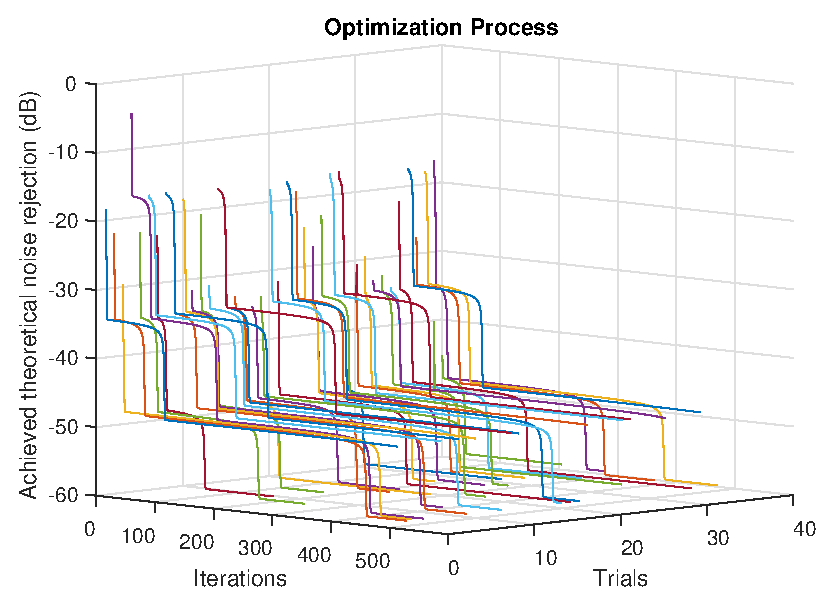
\includegraphics[width=3.45in]{opt-convergence}
	\caption{An example of the dependence of the iterative optimization scheme on initial conditions.} \label{fig:opt-convergence}
\end{figure}